\documentclass[]{article}
\usepackage{lmodern}
\usepackage{amssymb,amsmath}
\usepackage{ifxetex,ifluatex}
\usepackage{fixltx2e} % provides \textsubscript
\ifnum 0\ifxetex 1\fi\ifluatex 1\fi=0 % if pdftex
  \usepackage[T1]{fontenc}
  \usepackage[utf8]{inputenc}
\else % if luatex or xelatex
  \ifxetex
    \usepackage{mathspec}
  \else
    \usepackage{fontspec}
  \fi
  \defaultfontfeatures{Ligatures=TeX,Scale=MatchLowercase}
\fi
% use upquote if available, for straight quotes in verbatim environments
\IfFileExists{upquote.sty}{\usepackage{upquote}}{}
% use microtype if available
\IfFileExists{microtype.sty}{%
\usepackage{microtype}
\UseMicrotypeSet[protrusion]{basicmath} % disable protrusion for tt fonts
}{}
\usepackage[margin=1in]{geometry}
\usepackage{hyperref}
\hypersetup{unicode=true,
            pdftitle={DATA 621 - Homework 5},
            pdfauthor={Joshua Sturm},
            pdfborder={0 0 0},
            breaklinks=true}
\urlstyle{same}  % don't use monospace font for urls
\usepackage{graphicx,grffile}
\makeatletter
\def\maxwidth{\ifdim\Gin@nat@width>\linewidth\linewidth\else\Gin@nat@width\fi}
\def\maxheight{\ifdim\Gin@nat@height>\textheight\textheight\else\Gin@nat@height\fi}
\makeatother
% Scale images if necessary, so that they will not overflow the page
% margins by default, and it is still possible to overwrite the defaults
% using explicit options in \includegraphics[width, height, ...]{}
\setkeys{Gin}{width=\maxwidth,height=\maxheight,keepaspectratio}
\IfFileExists{parskip.sty}{%
\usepackage{parskip}
}{% else
\setlength{\parindent}{0pt}
\setlength{\parskip}{6pt plus 2pt minus 1pt}
}
\setlength{\emergencystretch}{3em}  % prevent overfull lines
\providecommand{\tightlist}{%
  \setlength{\itemsep}{0pt}\setlength{\parskip}{0pt}}
\setcounter{secnumdepth}{0}
% Redefines (sub)paragraphs to behave more like sections
\ifx\paragraph\undefined\else
\let\oldparagraph\paragraph
\renewcommand{\paragraph}[1]{\oldparagraph{#1}\mbox{}}
\fi
\ifx\subparagraph\undefined\else
\let\oldsubparagraph\subparagraph
\renewcommand{\subparagraph}[1]{\oldsubparagraph{#1}\mbox{}}
\fi

%%% Use protect on footnotes to avoid problems with footnotes in titles
\let\rmarkdownfootnote\footnote%
\def\footnote{\protect\rmarkdownfootnote}

%%% Change title format to be more compact
\usepackage{titling}

% Create subtitle command for use in maketitle
\newcommand{\subtitle}[1]{
  \posttitle{
    \begin{center}\large#1\end{center}
    }
}

\setlength{\droptitle}{-2em}
  \title{DATA 621 - Homework 5}
  \pretitle{\vspace{\droptitle}\centering\huge}
  \posttitle{\par}
  \author{Joshua Sturm}
  \preauthor{\centering\large\emph}
  \postauthor{\par}
  \predate{\centering\large\emph}
  \postdate{\par}
  \date{May 13, 2018}

\usepackage{booktabs}
\usepackage{longtable}
\usepackage{array}
\usepackage{multirow}
\usepackage[table]{xcolor}
\usepackage{wrapfig}
\usepackage{float}
\usepackage{colortbl}
\usepackage{pdflscape}
\usepackage{tabu}
\usepackage{threeparttable}
\usepackage{threeparttablex}
\usepackage[normalem]{ulem}
\usepackage{makecell}

\begin{document}
\maketitle

\hypertarget{objective}{%
\section{Objective}\label{objective}}

Your objective is to build a count regression model to predict the
number of cases of wine that will be sold given certain properties of
the wine. HINT: Sometimes, the fact that a variable is missing is
actually predictive of the target. You can only use the variables given
to you (or variables that you derive from the variables provided).

\hypertarget{data-exploration}{%
\section{1. Data Exploration}\label{data-exploration}}

\hypertarget{import-dataset}{%
\subsection{1.1 Import Dataset}\label{import-dataset}}

\hypertarget{data-dictionary}{%
\subsubsection{1.1.1 Data Dictionary}\label{data-dictionary}}

\begin{table}[H]
\centering\rowcolors{2}{gray!6}{white}

\resizebox{\linewidth}{!}{
\begin{tabular}{ll}
\hiderowcolors
\toprule
Variable Name & Definition\\
\midrule
\showrowcolors
TARGET & Number of Cases Purchased\\
AcidIndex & Proprietary method of testing total acidity of wine by using a weighted average\\
Alcohol & Alcohol Content\\
Chlorides & Chloride content of wine\\
CitricAcid & Citric Acid Content\\
\addlinespace
Density & Density of Wine\\
FixedAcidity & Fixed Acidity of Wine\\
FreeSulfurDioxide & Sulfur Dioxide content of wine\\
LabelAppeal & Marketing Score indicating the appeal of label design for consumers. High numbers suggest customers like the label design. Negative numbers suggest customers don't like the design\\
pH & pH of wine\\
\addlinespace
ResidualSugar & Residual Sugar of wine\\
STARS & Wine rating by a team of experts. 4 Stars = Excellent, 1 Star = Poor\\
Sulphates & Sulfate conten of wine\\
TotalSulfurDioxide & Total Sulfur Dioxide of Wine\\
VolatileAcidity & Volatile Acid content of wine\\
\bottomrule
\end{tabular}}
\rowcolors{2}{white}{white}
\end{table}

\hypertarget{data-structure}{%
\subsection{1.2 Data Structure}\label{data-structure}}

\begin{table}[H]
\centering\rowcolors{2}{gray!6}{white}

\resizebox{\linewidth}{!}{
\begin{tabular}{lrrrrrrrrrrrrr}
\hiderowcolors
\toprule
  & vars & n & mean & sd & median & trimmed & mad & min & max & range & skew & kurtosis & se\\
\midrule
\showrowcolors
TARGET & 1 & 12795 & 3.029074 & 1.926368 & 3.00000 & 3.053824 & 1.482600 & 0.00000 & 8.00000 & 8.00000 & -0.326301 & -0.877246 & 0.017030\\
AcidIndex & 2 & 12795 & 7.772724 & 1.323926 & 8.00000 & 7.643157 & 1.482600 & 4.00000 & 17.00000 & 13.00000 & 1.648496 & 5.190092 & 0.011704\\
Alcohol & 3 & 12142 & 10.489236 & 3.727819 & 10.40000 & 10.501826 & 2.372160 & -4.70000 & 26.50000 & 31.20000 & -0.030716 & 1.539495 & 0.033831\\
Chlorides & 4 & 12157 & 0.054822 & 0.318467 & 0.04600 & 0.054016 & 0.134917 & -1.17100 & 1.35100 & 2.52200 & 0.030427 & 1.788604 & 0.002888\\
CitricAcid & 5 & 12795 & 0.308413 & 0.862080 & 0.31000 & 0.310252 & 0.415128 & -3.24000 & 3.86000 & 7.10000 & -0.050307 & 1.837940 & 0.007621\\
\addlinespace
Density & 6 & 12795 & 0.994203 & 0.026538 & 0.99449 & 0.994213 & 0.009355 & 0.88809 & 1.09924 & 0.21115 & -0.018694 & 1.899959 & 0.000235\\
FixedAcidity & 7 & 12795 & 7.075717 & 6.317643 & 6.90000 & 7.073674 & 3.261720 & -18.10000 & 34.40000 & 52.50000 & -0.022586 & 1.674999 & 0.055852\\
FreeSulfurDioxide & 8 & 12148 & 30.845571 & 148.714558 & 30.00000 & 30.933488 & 56.338800 & -555.00000 & 623.00000 & 1178.00000 & 0.006393 & 1.836497 & 1.349277\\
LabelAppeal & 9 & 12795 & -0.009066 & 0.891089 & 0.00000 & -0.009964 & 1.482600 & -2.00000 & 2.00000 & 4.00000 & 0.008429 & -0.262292 & 0.007878\\
pH & 10 & 12400 & 3.207628 & 0.679687 & 3.20000 & 3.205571 & 0.385476 & 0.48000 & 6.13000 & 5.65000 & 0.044288 & 1.646268 & 0.006104\\
\addlinespace
ResidualSugar & 11 & 12179 & 5.418733 & 33.749379 & 3.90000 & 5.580041 & 15.715560 & -127.80000 & 141.15000 & 268.95000 & -0.053123 & 1.884692 & 0.305816\\
STARS & 12 & 9436 & 2.041755 & 0.902540 & 2.00000 & 1.971126 & 1.482600 & 1.00000 & 4.00000 & 3.00000 & 0.447235 & -0.692534 & 0.009291\\
Sulphates & 13 & 11585 & 0.527112 & 0.932129 & 0.50000 & 0.527145 & 0.444780 & -3.13000 & 4.24000 & 7.37000 & 0.005912 & 1.752566 & 0.008660\\
TotalSulfurDioxide & 14 & 12113 & 120.714233 & 231.913211 & 123.00000 & 120.889537 & 134.916600 & -823.00000 & 1057.00000 & 1880.00000 & -0.007179 & 1.674666 & 2.107170\\
VolatileAcidity & 15 & 12795 & 0.324104 & 0.784014 & 0.28000 & 0.324389 & 0.429954 & -2.79000 & 3.68000 & 6.47000 & 0.020380 & 1.832211 & 0.006931\\
\bottomrule
\end{tabular}}
\rowcolors{2}{white}{white}
\end{table}

The wine training dataset has 14 predictor variables, and 12795 cases.
Each case represents a commercially available brand of wine. We have a
sufficiently large sample size to perform (count) regression analysis on
the data.

\hypertarget{missing-data}{%
\subsubsection{1.2.1 Missing Data}\label{missing-data}}

\begin{verbatim}
##             TARGET          AcidIndex            Alcohol 
##                  0                  0                653 
##          Chlorides         CitricAcid            Density 
##                638                  0                  0 
##       FixedAcidity  FreeSulfurDioxide        LabelAppeal 
##                  0                647                  0 
##                 pH      ResidualSugar              STARS 
##                395                616               3359 
##          Sulphates TotalSulfurDioxide    VolatileAcidity 
##               1210                682                  0
\end{verbatim}

The training dataset is missing 8200 data points, with the bulk coming
from \texttt{STARS} and \texttt{Sulphates}.

\begin{verbatim}
## Observations: 12,795
## Variables: 15
## $ TARGET             <int> 3, 3, 5, 3, 4, 0, 0, 4, 3, 6, 0, 4, 3, 7, 4...
## $ AcidIndex          <int> 8, 7, 8, 6, 9, 11, 8, 7, 6, 8, 5, 10, 7, 8,...
## $ Alcohol            <dbl> 9.9, NA, 22.0, 6.2, 13.7, 15.4, 10.3, 11.6,...
## $ Chlorides          <dbl> -0.567, -0.425, 0.037, -0.425, NA, 0.556, 0...
## $ CitricAcid         <dbl> -0.98, -0.81, -0.88, 0.04, -1.26, 0.59, -0....
## $ Density            <dbl> 0.99280, 1.02792, 0.99518, 0.99640, 0.99457...
## $ FixedAcidity       <dbl> 3.2, 4.5, 7.1, 5.7, 8.0, 11.3, 7.7, 6.5, 14...
## $ FreeSulfurDioxide  <dbl> NA, 15, 214, 22, -167, -37, 287, 523, -213,...
## $ LabelAppeal        <int> 0, -1, -1, -1, 0, 0, 0, 1, 0, 0, 1, 0, 1, 2...
## $ pH                 <dbl> 3.33, 3.38, 3.12, 2.24, 3.12, 3.20, 3.49, 3...
## $ ResidualSugar      <dbl> 54.20, 26.10, 14.80, 18.80, 9.40, 2.20, 21....
## $ STARS              <int> 2, 3, 3, 1, 2, NA, NA, 3, NA, 4, 1, 2, 2, 3...
## $ Sulphates          <dbl> -0.59, 0.70, 0.48, 1.83, 1.77, 1.29, 1.21, ...
## $ TotalSulfurDioxide <dbl> 268, -327, 142, 115, 108, 15, 156, 551, NA,...
## $ VolatileAcidity    <dbl> 1.160, 0.160, 2.640, 0.385, 0.330, 0.320, 0...
\end{verbatim}

\hypertarget{summary-graphs}{%
\subsection{1.3 Summary Graphs}\label{summary-graphs}}

\hypertarget{boxplots}{%
\subsubsection{1.3.1 Boxplots}\label{boxplots}}

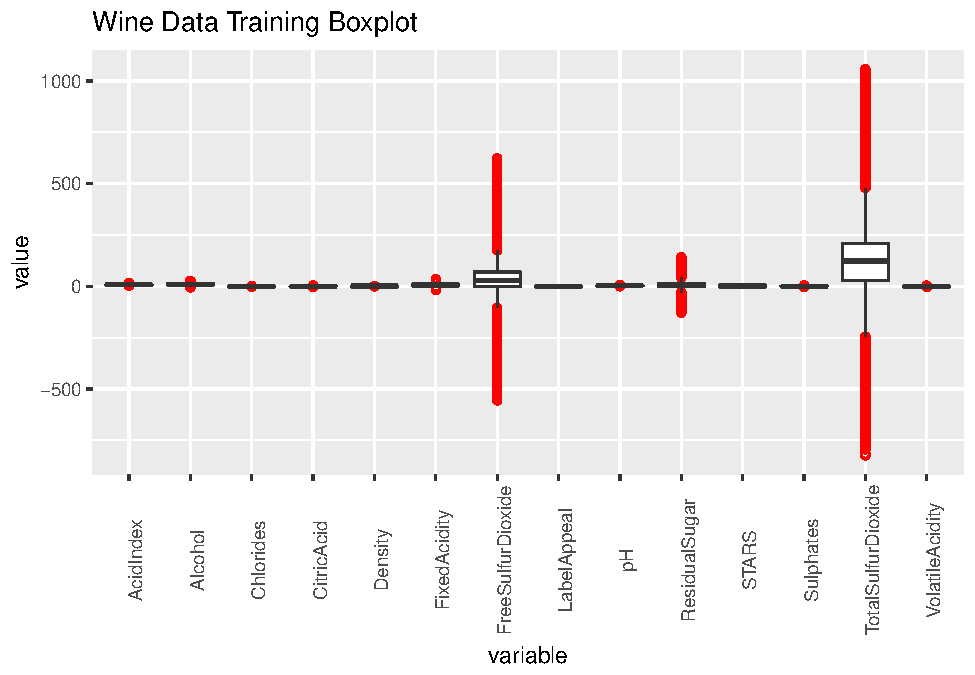
\includegraphics{DATA_621_Homework_5_files/figure-latex/summary-boxplot-1.pdf}

It's interesting to note that the outliers are nearly symmetrical for
every variable. This would suggest that the data is nearly normally
distributed.

\hypertarget{histograms}{%
\subsubsection{1.3.2 Histograms}\label{histograms}}

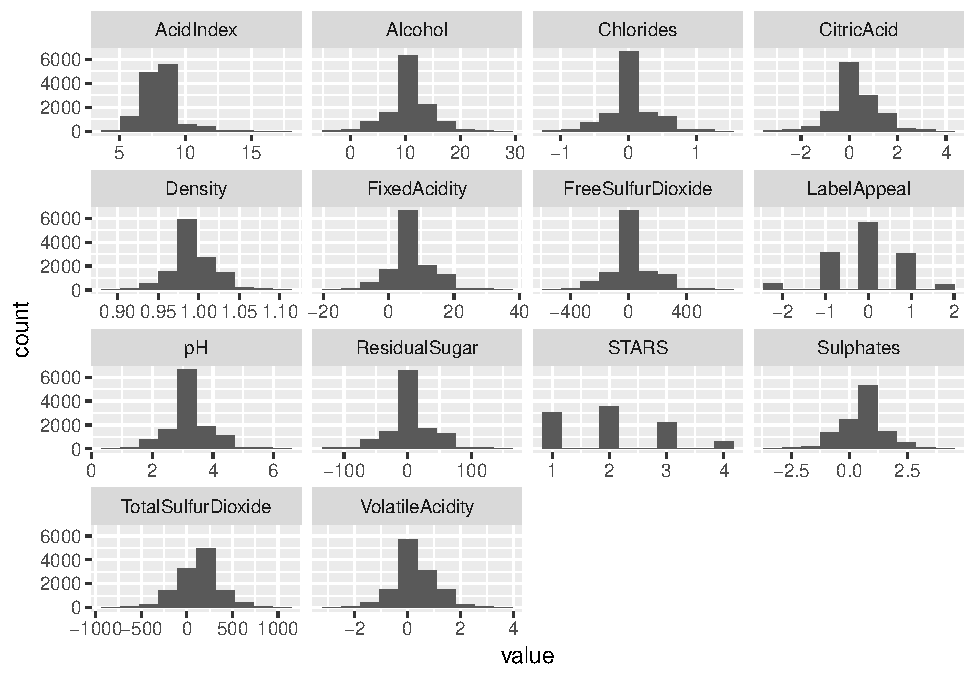
\includegraphics{DATA_621_Homework_5_files/figure-latex/summary-histogram-1.pdf}

The histograms confirm that the data is nearly normal.

\hypertarget{correlation}{%
\subsubsection{1.3.3 Correlation}\label{correlation}}

\hypertarget{correlation-heatmap}{%
\paragraph{1.3.3.1 Correlation Heatmap}\label{correlation-heatmap}}

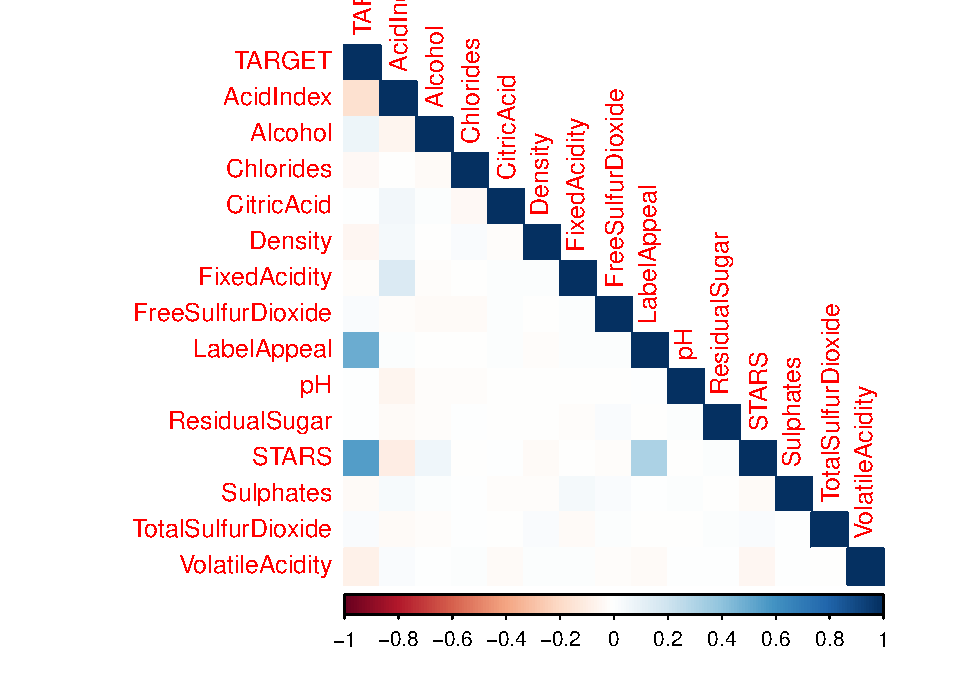
\includegraphics{DATA_621_Homework_5_files/figure-latex/summary-correlation-heatmap-1.pdf}

\hypertarget{correlation-with-response-table}{%
\paragraph{1.3.3.2 Correlation (with response)
table}\label{correlation-with-response-table}}

\begin{table}[H]
\centering\rowcolors{2}{gray!6}{white}

\begin{tabular}{lll}
\hiderowcolors
\toprule
  & P-value & Correlation with response\\
\midrule
\showrowcolors
TARGET & 0 & 1\\
AcidIndex & 9.37395581821143e-176 & -0.167643064841741\\
Alcohol & 7.67392068595044e-12 & 0.0737771083653496\\
Chlorides & 0.0000244355000721859 & -0.0304301331416401\\
CitricAcid & 0.325959600816776 & 0.00234504903198721\\
\addlinespace
Density & 0.000058585480680226 & -0.0475989086144533\\
FixedAcidity & 2.91172690566348e-08 & -0.0125380998033961\\
FreeSulfurDioxide & 0.00000135147274457202 & 0.0226398054129899\\
LabelAppeal & 0 & 0.49794647956962\\
pH & 0.29296223052554 & 0.000219855723603457\\
\addlinespace
ResidualSugar & 0.0687760354246013 & 0.00351959992133455\\
STARS & 0 & 0.554685722299802\\
Sulphates & 0.0000288130617993951 & -0.0212203782563951\\
TotalSulfurDioxide & 1.43765745126653e-08 & 0.0216020725627316\\
VolatileAcidity & 8.0718402641318e-24 & -0.075997876547476\\
\bottomrule
\end{tabular}
\rowcolors{2}{white}{white}
\end{table}

\texttt{STARS} and \texttt{LabelAppeal} are the most significantly
correlated with the response variable. I find it amusing that the
superficial aspects have a bigger impact on sales than the actual
qualities of the wine.

\hypertarget{data-preparation}{%
\section{2. Data Preparation}\label{data-preparation}}

\hypertarget{missing-values}{%
\subsection{2.1 Missing Values}\label{missing-values}}

As noted earlier in \protect\hyperlink{missing-data}{Section 1.2.1},
there are several variables with a significant number of missing cases.
The \texttt{STARS} variable has the most missing cases. Based on the
definition found in the data dictionary, the number indicates the
quality rated by a panel of experts. Luckily, there are no 0 scores, so
I'll convert this variable to an ordered factor, with the missing cases
taking on a value of 0. The remaining variables with missing cases will
be imputated using the \texttt{Hmisc} package.

\hypertarget{negative-values}{%
\subsection{2.2 Negative Values}\label{negative-values}}

Going by the definitions found in the data dictionary, most, if not all,
variables cannot possibly take on negative values. However, since the
dataset is nearly normal, it's unlikely that it's due to an entry error.
Without knowing how the data was recorded and entered, I will not be
altering any of the negative values in the dataset, and will proceed to
build the models using them as is.

\hypertarget{build-models}{%
\section{3. Build Models}\label{build-models}}

In each case, I will build two models - one using the raw dataset, the
other using our transformed one.

\hypertarget{poisson-model-1}{%
\subsection{3.1 Poisson Model 1}\label{poisson-model-1}}

\begin{verbatim}
## 
## Call:
## glm(formula = TARGET ~ ., family = "poisson", data = wine.t)
## 
## Deviance Residuals: 
##    Min      1Q  Median      3Q     Max  
## -3.216  -0.273   0.062   0.373   1.683  
## 
## Coefficients:
##                      Estimate Std. Error z value Pr(>|z|)    
## (Intercept)         1.5934011  0.2505767    6.36    2e-10 ***
## AcidIndex          -0.0487011  0.0059026   -8.25   <2e-16 ***
## Alcohol             0.0039476  0.0017707    2.23   0.0258 *  
## Chlorides          -0.0300746  0.0205567   -1.46   0.1435    
## CitricAcid         -0.0007259  0.0075750   -0.10   0.9237    
## Density            -0.3724851  0.2461767   -1.51   0.1303    
## FixedAcidity        0.0003293  0.0010529    0.31   0.7545    
## FreeSulfurDioxide   0.0000673  0.0000440    1.53   0.1262    
## LabelAppeal         0.1771425  0.0079540   22.27   <2e-16 ***
## pH                 -0.0046612  0.0095981   -0.49   0.6272    
## ResidualSugar      -0.0000614  0.0001941   -0.32   0.7517    
## STARS               0.1871147  0.0074868   24.99   <2e-16 ***
## Sulphates          -0.0051638  0.0070514   -0.73   0.4640    
## TotalSulfurDioxide  0.0000208  0.0000286    0.73   0.4662    
## VolatileAcidity    -0.0256013  0.0083530   -3.06   0.0022 ** 
## ---
## Signif. codes:  0 '***' 0.001 '**' 0.01 '*' 0.05 '.' 0.1 ' ' 1
## 
## (Dispersion parameter for poisson family taken to be 1)
## 
##     Null deviance: 5844.1  on 6435  degrees of freedom
## Residual deviance: 4009.1  on 6421  degrees of freedom
##   (6359 observations deleted due to missingness)
## AIC: 23172
## 
## Number of Fisher Scoring iterations: 5
## [1] "RMSE = 0.373017203364726"
\end{verbatim}

\hypertarget{poisson-model-1-interpretation}{%
\subsubsection{3.1.1 Poisson Model 1
Interpretation}\label{poisson-model-1-interpretation}}

The model suggest there are many variables that are not significantly
contributing toward predicting the target variable.

The model has an AIC (Akaike information criterion) of 23171.75, and a
BIC (Bayesian information criterion) of 23273.29.

With a Null deviance of 5844.06, and a Residual deviance of 4009.14, we
get a difference of 1834.91.

\hypertarget{poisson-model-2}{%
\subsection{3.2 Poisson Model 2}\label{poisson-model-2}}

\begin{verbatim}
## 
## Call:
## glm(formula = TARGET ~ ., family = "poisson", data = imputed.training)
## 
## Deviance Residuals: 
##    Min      1Q  Median      3Q     Max  
## -3.229  -0.652  -0.003   0.444   3.690  
## 
## Coefficients:
##                      Estimate Std. Error z value Pr(>|z|)    
## (Intercept)         0.2911933  0.3711928    0.78  0.43276    
## AcidIndex5         -0.1612419  0.3226409   -0.50  0.61725    
## AcidIndex6         -0.1178142  0.3172205   -0.37  0.71034    
## AcidIndex7         -0.1521719  0.3169681   -0.48  0.63117    
## AcidIndex8         -0.1837017  0.3170140   -0.58  0.56227    
## AcidIndex9         -0.2944243  0.3173478   -0.93  0.35353    
## AcidIndex10        -0.4510683  0.3184496   -1.42  0.15664    
## AcidIndex11        -0.8142054  0.3220420   -2.53  0.01146 *  
## AcidIndex12        -0.8279904  0.3277075   -2.53  0.01152 *  
## AcidIndex13        -0.6656454  0.3306041   -2.01  0.04407 *  
## AcidIndex14        -0.7645931  0.3432296   -2.23  0.02590 *  
## AcidIndex15        -0.3323601  0.4038546   -0.82  0.41053    
## AcidIndex16        -0.9794886  0.5484548   -1.79  0.07411 .  
## AcidIndex17        -1.1956613  0.5485977   -2.18  0.02930 *  
## Alcohol             0.0037531  0.0013756    2.73  0.00636 ** 
## Chlorides          -0.0340748  0.0160782   -2.12  0.03406 *  
## CitricAcid          0.0047149  0.0058964    0.80  0.42393    
## Density            -0.2778312  0.1917960   -1.45  0.14746    
## FixedAcidity        0.0001361  0.0008203    0.17  0.86823    
## FreeSulfurDioxide   0.0000807  0.0000343    2.35  0.01858 *  
## LabelAppeal-1       0.2394029  0.0379989    6.30  3.0e-10 ***
## LabelAppeal0        0.4297595  0.0370630   11.60  < 2e-16 ***
## LabelAppeal1        0.5630285  0.0377096   14.93  < 2e-16 ***
## LabelAppeal2        0.6992452  0.0424502   16.47  < 2e-16 ***
## pH                 -0.0090289  0.0075156   -1.20  0.22961    
## ResidualSugar       0.0000390  0.0001515    0.26  0.79683    
## STARS1              0.7550021  0.0195726   38.57  < 2e-16 ***
## STARS2              1.0736578  0.0182725   58.76  < 2e-16 ***
## STARS3              1.1918268  0.0192433   61.93  < 2e-16 ***
## STARS4              1.3126656  0.0243336   53.94  < 2e-16 ***
## Sulphates          -0.0072465  0.0054546   -1.33  0.18400    
## TotalSulfurDioxide  0.0000738  0.0000221    3.34  0.00085 ***
## VolatileAcidity    -0.0295346  0.0065347   -4.52  6.2e-06 ***
## ---
## Signif. codes:  0 '***' 0.001 '**' 0.01 '*' 0.05 '.' 0.1 ' ' 1
## 
## (Dispersion parameter for poisson family taken to be 1)
## 
##     Null deviance: 22861  on 12794  degrees of freedom
## Residual deviance: 13535  on 12762  degrees of freedom
## AIC: 45543
## 
## Number of Fisher Scoring iterations: 6
## [1] "RMSE = 0.75913775554001"
\end{verbatim}

\hypertarget{poisson-model-2-interpretation}{%
\subsubsection{3.2.1 Poisson Model 2
Interpretation}\label{poisson-model-2-interpretation}}

This model has an AIC (Akaike information criterion) of 45542.95, and a
BIC (Bayesian information criterion) of 45789.03.

With a Null deviance of 22860.89, and a Residual deviance of 13534.93,
we get a difference of 9325.96.

\hypertarget{poisson-results}{%
\subsection{3.3 Poisson Results}\label{poisson-results}}

Interestingly, the model using the raw dataset outperformed the modified
one. Nevertheless, the model results are subpar, and neither should be
used in production.

\hypertarget{negative-binomial-model-1}{%
\subsection{3.4 Negative Binomial Model
1}\label{negative-binomial-model-1}}

\begin{verbatim}
## 
## Call:
## glm.nb(formula = TARGET ~ ., data = wine.t, init.theta = 140197.922, 
##     link = log)
## 
## Deviance Residuals: 
##    Min      1Q  Median      3Q     Max  
## -3.216  -0.273   0.062   0.373   1.683  
## 
## Coefficients:
##                      Estimate Std. Error z value Pr(>|z|)    
## (Intercept)         1.5934044  0.2505802    6.36    2e-10 ***
## AcidIndex          -0.0487013  0.0059026   -8.25   <2e-16 ***
## Alcohol             0.0039476  0.0017707    2.23   0.0258 *  
## Chlorides          -0.0300748  0.0205569   -1.46   0.1435    
## CitricAcid         -0.0007259  0.0075751   -0.10   0.9237    
## Density            -0.3724871  0.2461802   -1.51   0.1303    
## FixedAcidity        0.0003293  0.0010529    0.31   0.7545    
## FreeSulfurDioxide   0.0000673  0.0000440    1.53   0.1262    
## LabelAppeal         0.1771427  0.0079541   22.27   <2e-16 ***
## pH                 -0.0046613  0.0095982   -0.49   0.6272    
## ResidualSugar      -0.0000614  0.0001941   -0.32   0.7517    
## STARS               0.1871151  0.0074869   24.99   <2e-16 ***
## Sulphates          -0.0051639  0.0070515   -0.73   0.4640    
## TotalSulfurDioxide  0.0000208  0.0000286    0.73   0.4662    
## VolatileAcidity    -0.0256015  0.0083531   -3.06   0.0022 ** 
## ---
## Signif. codes:  0 '***' 0.001 '**' 0.01 '*' 0.05 '.' 0.1 ' ' 1
## 
## (Dispersion parameter for Negative Binomial(140198) family taken to be 1)
## 
##     Null deviance: 5843.9  on 6435  degrees of freedom
## Residual deviance: 4009.1  on 6421  degrees of freedom
##   (6359 observations deleted due to missingness)
## AIC: 23174
## 
## Number of Fisher Scoring iterations: 1
## 
## 
##               Theta:  140198 
##           Std. Err.:  234985 
## Warning while fitting theta: iteration limit reached 
## 
##  2 x log-likelihood:  -23141.9
## [1] "RMSE = 0.373017366291372"
\end{verbatim}

\hypertarget{nb-model-1-interpretation}{%
\subsubsection{3.4.1 NB Model 1
Interpretation}\label{nb-model-1-interpretation}}

The model has an AIC (Akaike information criterion) of 23173.85, and a
BIC (Bayesian information criterion) of 23282.17.

With a Null deviance of 5843.95, and a Residual deviance of 4009.08, we
get a difference of 1834.87.

\hypertarget{negative-binomial-model-2}{%
\subsection{3.5 Negative Binomial Model
2}\label{negative-binomial-model-2}}

\begin{verbatim}
## 
## Call:
## glm.nb(formula = TARGET ~ ., data = imputed.training, init.theta = 40933.36399, 
##     link = log)
## 
## Deviance Residuals: 
##    Min      1Q  Median      3Q     Max  
## -3.229  -0.652  -0.003   0.444   3.690  
## 
## Coefficients:
##                      Estimate Std. Error z value Pr(>|z|)    
## (Intercept)         0.2912221  0.3712137    0.78  0.43274    
## AcidIndex5         -0.1612617  0.3226604   -0.50  0.61722    
## AcidIndex6         -0.1178325  0.3172397   -0.37  0.71032    
## AcidIndex7         -0.1521908  0.3169873   -0.48  0.63114    
## AcidIndex8         -0.1837214  0.3170333   -0.58  0.56225    
## AcidIndex9         -0.2944475  0.3173671   -0.93  0.35352    
## AcidIndex10        -0.4510938  0.3184688   -1.42  0.15665    
## AcidIndex11        -0.8142353  0.3220611   -2.53  0.01146 *  
## AcidIndex12        -0.8280219  0.3277265   -2.53  0.01152 *  
## AcidIndex13        -0.6656752  0.3306232   -2.01  0.04407 *  
## AcidIndex14        -0.7646198  0.3432484   -2.23  0.02591 *  
## AcidIndex15        -0.3323861  0.4038745   -0.82  0.41051    
## AcidIndex16        -0.9795247  0.5484725   -1.79  0.07411 .  
## AcidIndex17        -1.1956999  0.5486143   -2.18  0.02930 *  
## Alcohol             0.0037530  0.0013756    2.73  0.00637 ** 
## Chlorides          -0.0340759  0.0160790   -2.12  0.03407 *  
## CitricAcid          0.0047150  0.0058967    0.80  0.42394    
## Density            -0.2778344  0.1918047   -1.45  0.14747    
## FixedAcidity        0.0001361  0.0008204    0.17  0.86824    
## FreeSulfurDioxide   0.0000807  0.0000343    2.35  0.01858 *  
## LabelAppeal-1       0.2394025  0.0379998    6.30  3.0e-10 ***
## LabelAppeal0        0.4297580  0.0370639   11.60  < 2e-16 ***
## LabelAppeal1        0.5630250  0.0377105   14.93  < 2e-16 ***
## LabelAppeal2        0.6992413  0.0424516   16.47  < 2e-16 ***
## pH                 -0.0090298  0.0075159   -1.20  0.22959    
## ResidualSugar       0.0000390  0.0001515    0.26  0.79681    
## STARS1              0.7550011  0.0195730   38.57  < 2e-16 ***
## STARS2              1.0736573  0.0182729   58.76  < 2e-16 ***
## STARS3              1.1918270  0.0192438   61.93  < 2e-16 ***
## STARS4              1.3126669  0.0243347   53.94  < 2e-16 ***
## Sulphates          -0.0072468  0.0054548   -1.33  0.18401    
## TotalSulfurDioxide  0.0000739  0.0000221    3.34  0.00085 ***
## VolatileAcidity    -0.0295354  0.0065350   -4.52  6.2e-06 ***
## ---
## Signif. codes:  0 '***' 0.001 '**' 0.01 '*' 0.05 '.' 0.1 ' ' 1
## 
## (Dispersion parameter for Negative Binomial(40933.4) family taken to be 1)
## 
##     Null deviance: 22860  on 12794  degrees of freedom
## Residual deviance: 13534  on 12762  degrees of freedom
## AIC: 45545
## 
## Number of Fisher Scoring iterations: 1
## 
## 
##               Theta:  40933 
##           Std. Err.:  34321 
## Warning while fitting theta: iteration limit reached 
## 
##  2 x log-likelihood:  -45477.4
## [1] "RMSE = 0.759138253409953"
\end{verbatim}

\hypertarget{nb-model-2-interpretation}{%
\subsubsection{3.5.1 NB Model 2
Interpretation}\label{nb-model-2-interpretation}}

The model has an AIC (Akaike information criterion) of 45545.37, and a
BIC (Bayesian information criterion) of 45798.9.

With a Null deviance of 22859.73, and a Residual deviance of 13534.4, we
get a difference of 9325.33.

\begin{verbatim}
## 
## Call:
## zeroinfl(formula = TARGET ~ ., data = imputed.training, dist = "negbin")
## 
## Pearson residuals:
##      Min       1Q   Median       3Q      Max 
## -2.28291 -0.42582 -0.00089  0.38071  5.13214 
## 
## Count model coefficients (negbin with log link):
##                       Estimate  Std. Error z value  Pr(>|z|)    
## (Intercept)         0.58893768  0.39011751    1.51    0.1311    
## AcidIndex5          0.02618191  0.33882130    0.08    0.9384    
## AcidIndex6          0.05548817  0.33355532    0.17    0.8679    
## AcidIndex7          0.02920359  0.33330386    0.09    0.9302    
## AcidIndex8          0.01461506  0.33335117    0.04    0.9650    
## AcidIndex9         -0.01936724  0.33367803   -0.06    0.9537    
## AcidIndex10        -0.08724828  0.33483525   -0.26    0.7944    
## AcidIndex11        -0.08110035  0.33859577   -0.24    0.8107    
## AcidIndex12        -0.00661812  0.34458496   -0.02    0.9847    
## AcidIndex13         0.05855686  0.34737745    0.17    0.8661    
## AcidIndex14         0.06983987  0.36062939    0.19    0.8464    
## AcidIndex15         0.12702915  0.42188126    0.30    0.7633    
## AcidIndex16         0.20210948  0.55859074    0.36    0.7175    
## AcidIndex17        -0.14351369  0.56032154   -0.26    0.7979    
## Alcohol             0.00663385  0.00140229    4.73 0.0000022 ***
## Chlorides          -0.02196073  0.01647990   -1.33    0.1827    
## CitricAcid          0.00053731  0.00601715    0.09    0.9288    
## Density            -0.24938851  0.19775215   -1.26    0.2073    
## FixedAcidity        0.00035009  0.00084160    0.42    0.6774    
## FreeSulfurDioxide   0.00002178  0.00003461    0.63    0.5292    
## LabelAppeal-1       0.43704623  0.04132163   10.58   < 2e-16 ***
## LabelAppeal0        0.72518557  0.04039369   17.95   < 2e-16 ***
## LabelAppeal1        0.91538511  0.04106778   22.29   < 2e-16 ***
## LabelAppeal2        1.07513809  0.04559694   23.58   < 2e-16 ***
## pH                  0.00469166  0.00771761    0.61    0.5432    
## ResidualSugar      -0.00003796  0.00015505   -0.24    0.8066    
## STARS1              0.05983667  0.02113752    2.83    0.0046 ** 
## STARS2              0.18135607  0.01975545    9.18   < 2e-16 ***
## STARS3              0.27780696  0.02068764   13.43   < 2e-16 ***
## STARS4              0.37682280  0.02561429   14.71   < 2e-16 ***
## Sulphates           0.00027776  0.00559292    0.05    0.9604    
## TotalSulfurDioxide -0.00000939  0.00002202   -0.43    0.6698    
## VolatileAcidity    -0.01229560  0.00670986   -1.83    0.0669 .  
## Log(theta)         20.85755836          NA      NA        NA    
## 
## Zero-inflation model coefficients (binomial with logit link):
##                       Estimate  Std. Error z value Pr(>|z|)    
## (Intercept)          -4.616579    2.137309   -2.16  0.03077 *  
## AcidIndex5            0.952393    1.716154    0.55  0.57892    
## AcidIndex6            0.654080    1.656172    0.39  0.69289    
## AcidIndex7            0.806160    1.653080    0.49  0.62578    
## AcidIndex8            1.024494    1.653249    0.62  0.53547    
## AcidIndex9            1.701720    1.655242    1.03  0.30391    
## AcidIndex10           1.953469    1.658346    1.18  0.23881    
## AcidIndex11           3.394177    1.669406    2.03  0.04204 *  
## AcidIndex12           3.397201    1.686405    2.01  0.04396 *  
## AcidIndex13           3.920553    1.723857    2.27  0.02295 *  
## AcidIndex14           3.086898    1.712461    1.80  0.07145 .  
## AcidIndex15           2.369111    1.919278    1.23  0.21706    
## AcidIndex16          15.862903  515.393962    0.03  0.97545    
## AcidIndex17          14.739564  581.609730    0.03  0.97978    
## Alcohol               0.026950    0.009267    2.91  0.00363 ** 
## Chlorides             0.066535    0.108317    0.61  0.53904    
## CitricAcid           -0.025002    0.039852   -0.63  0.53043    
## Density               0.818279    1.317146    0.62  0.53443    
## FixedAcidity          0.000827    0.005533    0.15  0.88123    
## FreeSulfurDioxide    -0.000646    0.000236   -2.74  0.00607 ** 
## LabelAppeal-1         1.454858    0.324471    4.48  7.3e-06 ***
## LabelAppeal0          2.201277    0.321834    6.84  7.9e-12 ***
## LabelAppeal1          2.918416    0.327503    8.91  < 2e-16 ***
## LabelAppeal2          3.380579    0.380114    8.89  < 2e-16 ***
## pH                    0.190045    0.050645    3.75  0.00018 ***
## ResidualSugar        -0.000830    0.001022   -0.81  0.41657    
## STARS1               -2.085709    0.076960  -27.10  < 2e-16 ***
## STARS2               -5.837879    0.334343  -17.46  < 2e-16 ***
## STARS3              -28.690015  693.309579   -0.04  0.96699    
## STARS4              -21.405472 1039.233168   -0.02  0.98357    
## Sulphates             0.084112    0.036422    2.31  0.02092 *  
## TotalSulfurDioxide   -0.000916    0.000149   -6.13  8.6e-10 ***
## VolatileAcidity       0.177338    0.043644    4.06  4.8e-05 ***
## ---
## Signif. codes:  0 '***' 0.001 '**' 0.01 '*' 0.05 '.' 0.1 ' ' 1 
## 
## Theta = 1143727342.244 
## Number of iterations in BFGS optimization: 94 
## Log-likelihood: -2.03e+04 on 67 Df
## [1] "RMSE = 1.26029677215806"
\end{verbatim}

\hypertarget{negative-binomial-results}{%
\subsection{3.6 Negative Binomial
Results}\label{negative-binomial-results}}

Both these models performed nearly identically to the Poisson models.
However, the zero-inflated negative binomial out-performed both.

\hypertarget{linear-model-1}{%
\subsection{3.7 Linear Model 1}\label{linear-model-1}}

\begin{verbatim}
## 
## Call:
## lm(formula = TARGET ~ ., data = wine.t)
## 
## Residuals:
##    Min     1Q Median     3Q    Max 
## -5.061 -0.514  0.124  0.717  3.242 
## 
## Coefficients:
##                      Estimate Std. Error t value  Pr(>|t|)    
## (Intercept)         4.5629928  0.5530057    8.25   < 2e-16 ***
## AcidIndex          -0.1648540  0.0123519  -13.35   < 2e-16 ***
## Alcohol             0.0165298  0.0038874    4.25 0.0000215 ***
## Chlorides          -0.1133879  0.0454596   -2.49     0.013 *  
## CitricAcid         -0.0048361  0.0167530   -0.29     0.773    
## Density            -1.2808964  0.5435008   -2.36     0.018 *  
## FixedAcidity        0.0016850  0.0023191    0.73     0.468    
## FreeSulfurDioxide   0.0002264  0.0000971    2.33     0.020 *  
## LabelAppeal         0.6441786  0.0174350   36.95   < 2e-16 ***
## pH                 -0.0094405  0.0212141   -0.45     0.656    
## ResidualSugar      -0.0002513  0.0004276   -0.59     0.557    
## STARS               0.7278225  0.0170967   42.57   < 2e-16 ***
## Sulphates          -0.0172718  0.0155774   -1.11     0.268    
## TotalSulfurDioxide  0.0000781  0.0000629    1.24     0.214    
## VolatileAcidity    -0.0946637  0.0184578   -5.13 0.0000003 ***
## ---
## Signif. codes:  0 '***' 0.001 '**' 0.01 '*' 0.05 '.' 0.1 ' ' 1
## 
## Residual standard error: 1.15 on 6421 degrees of freedom
##   (6359 observations deleted due to missingness)
## Multiple R-squared:  0.445,  Adjusted R-squared:  0.444 
## F-statistic:  368 on 14 and 6421 DF,  p-value: <2e-16
\end{verbatim}

\hypertarget{linear-model-2}{%
\subsection{3.8 Linear Model 2}\label{linear-model-2}}

\begin{verbatim}
## 
## Call:
## lm(formula = TARGET ~ ., data = imputed.training)
## 
## Residuals:
##    Min     1Q Median     3Q    Max 
## -4.976 -0.859  0.034  0.840  6.094 
## 
## Coefficients:
##                      Estimate Std. Error t value Pr(>|t|)    
## (Intercept)         1.7730958  0.8688303    2.04  0.04129 *  
## AcidIndex5         -0.3214870  0.7682252   -0.42  0.67560    
## AcidIndex6         -0.2096532  0.7543669   -0.28  0.78108    
## AcidIndex7         -0.3125649  0.7537377   -0.41  0.67838    
## AcidIndex8         -0.4199441  0.7538060   -0.56  0.57747    
## AcidIndex9         -0.7246396  0.7543785   -0.96  0.33678    
## AcidIndex10        -1.0326465  0.7556415   -1.37  0.17178    
## AcidIndex11        -1.5088756  0.7580225   -1.99  0.04655 *  
## AcidIndex12        -1.5261471  0.7624395   -2.00  0.04534 *  
## AcidIndex13        -1.5445329  0.7698757   -2.01  0.04485 *  
## AcidIndex14        -1.3911532  0.7775546   -1.79  0.07362 .  
## AcidIndex15        -0.6970514  0.8835118   -0.79  0.43015    
## AcidIndex16        -1.7663108  0.9532400   -1.85  0.06391 .  
## AcidIndex17        -1.8944876  0.9011988   -2.10  0.03556 *  
## Alcohol             0.0118595  0.0031085    3.82  0.00014 ***
## Chlorides          -0.1089252  0.0363598   -3.00  0.00274 ** 
## CitricAcid          0.0171582  0.0134119    1.28  0.20081    
## Density            -0.8356750  0.4350987   -1.92  0.05480 .  
## FixedAcidity        0.0007257  0.0018558    0.39  0.69576    
## FreeSulfurDioxide   0.0002421  0.0000779    3.11  0.00189 ** 
## LabelAppeal-1       0.3658647  0.0627490    5.83  5.7e-09 ***
## LabelAppeal0        0.8340821  0.0611850   13.63  < 2e-16 ***
## LabelAppeal1        1.3005447  0.0639309   20.34  < 2e-16 ***
## LabelAppeal2        1.8893947  0.0841938   22.44  < 2e-16 ***
## pH                 -0.0246095  0.0169724   -1.45  0.14709    
## ResidualSugar       0.0001727  0.0003433    0.50  0.61485    
## STARS1              1.3469248  0.0329336   40.90  < 2e-16 ***
## STARS2              2.3831232  0.0320302   74.40  < 2e-16 ***
## STARS3              2.9449302  0.0370842   79.41  < 2e-16 ***
## STARS4              3.6330551  0.0591556   61.42  < 2e-16 ***
## Sulphates          -0.0188011  0.0123180   -1.53  0.12696    
## TotalSulfurDioxide  0.0002131  0.0000499    4.27  2.0e-05 ***
## VolatileAcidity    -0.0938528  0.0147574   -6.36  2.1e-10 ***
## ---
## Signif. codes:  0 '***' 0.001 '**' 0.01 '*' 0.05 '.' 0.1 ' ' 1
## 
## Residual standard error: 1.3 on 12762 degrees of freedom
## Multiple R-squared:  0.544,  Adjusted R-squared:  0.543 
## F-statistic:  475 on 32 and 12762 DF,  p-value: <2e-16
\end{verbatim}

\hypertarget{model-selection-and-prediction}{%
\section{4. Model Selection and
Prediction}\label{model-selection-and-prediction}}

The linear models were the only scenario where the modified dataset
outperformed the raw one. The second linear model was the best performed
out of all 7 models, with the zero-inflated negative binomial coming in
second. I will be using the zinb to make predictions on the evaluation
dataset.

Below is a sample of the prediction results.

\begin{verbatim}
##    ID Predicted
## 1   1  1.826236
## 2   2  4.034349
## 3   3  2.510621
## 4   4  2.405798
## 5   5  0.779140
## 6   6  5.670287
## 7   7  3.965553
## 8   8  1.398592
## 9   9  0.201435
## 10 10  1.534990
##           used  (Mb) gc trigger  (Mb) max used  (Mb)
## Ncells 2120753 113.3    3814665 203.8  3814665 203.8
## Vcells 7670280  58.6   17827294 136.1 17827139 136.1
\end{verbatim}


\end{document}
